%
% Copyright 2018 Joel Feldman, Andrew Rechnitzer and Elyse Yeager.
% This work is licensed under a Creative Commons Attribution-NonCommercial-ShareAlike 4.0 International License.
% https://creativecommons.org/licenses/by-nc-sa/4.0/
%

\questionheader{ex:s3.4.8}


%%%%%%%%%%%%%%%%%%
\subsection*{\Conceptual}
%%%%%%%%%%%%%%%%%%


\begin{Mquestion}
Suppose $f(x)$ is a function that we approximated by $F(x)$. Further, suppose
 $f(10)=-3$, while our approximation was $F(10)=5$. Let $R(x)=f(x)-F(x)$.
 \begin{enumerate}[(a)]
 \item True or false: $|R(10)| \leq 7$
 \item True or false: $|R(10)| \leq 8$
 \item True or false: $|R(10)| \leq 9$
  \item True or false: $|R(10)| \leq 100$
 \end{enumerate}
\end{Mquestion}
\begin{hint}
$R(10)=f(10)-F(10)=-3-5$
\end{hint}
\begin{answer} (a) False \qquad
(b) True \qquad
(c) True \qquad
(d) True
\end{answer}
\begin{solution}
From the given information,
\[|R(10)|=|f(10)-F(10)|=|-3-5|=|-8|=8\]
So, (a) is false (since 8 is not less than or equal to 7), while (b), (c), and (d) are true.

Remark: $R(x)$ is the error in our approximation. As mentioned in the text, we almost never know $R$ exactly, but we can give a bound. We don't need the tightest bound--just a reasonable one that is easy to calculate. If we were dealing with real functions and approximations, we might not know that $|R(10)|=8$, but if we knew it was at most 9, that would be a pretty decent approximation.

 Often in this section, we will make simplifying assumptions to get a bound that is easy to calculate. But, don't go overboard! It is a true statement to say that our absolute error is at most 100, but this statement would probably not be very helpful as a bound.
\end{solution}



%\begin{question}
%Let $f(x)=(x-3)^2$.
%\begin{enumerate}[(a)]
%\item Give the constant approximation $T_0(x)$ of $f(x)$ about $x=0$.
%\item Sketch $f(x)$, and the secant line from $(0,f(0))$ to $(3,f(3))$.
%\item On your sketch, locate an approximate value of $c$ such that $f'(c)$ gives the %slope of the secant line you drew (from $x=0$ to $x=3$).
%\item Solve the equation $f(3)-T_0(3)=f'(c)(3-0)$ for $c$. Is this close to what you %marked on your sketch?
%\end{enumerate}
%\end{question}
%\begin{hint}
%\end{hint}
%\begin{answer}
%\end{answer}
%\begin{solution}
%\end{solution}


\begin{Mquestion}
Let $f(x)=e^x$, and let $T_3(x)$ be the third-degree Maclaurin polynomial for $f(x)$,
\[T_3(x)=1+x+\frac{1}{2}x^2+\frac{1}{3!}x^3\]
Use Equation~\ref*{eq:taylorErrorN} to give a reasonable bound on the error $|f(2)-T_3(2)|$.
Then, find the error $|f(2)-T_3(2)|$ using a calculator.
\end{Mquestion}
\begin{hint}
Equation~\ref*{eq:taylorErrorN} tells us
\[|f(2)-T_3(2)| = \left|\frac{f^{(4)}(c)}{4!}(2-0)^4\right|\]
for some $c$ strictly between 0 and 2.
\end{hint}
\begin{answer}
Equation~\ref*{eq:taylorErrorN} gives us the bound $|f(2)-T_3(2)|<6$. A calculator tells us actually $|f(2)-T_3(2)|\approx 1.056$.
\end{answer}
\begin{solution}
Equation~\ref*{eq:taylorErrorN} tells us that, when $T_n(x)$ is the $n$th degree Taylor polynomial for a function $f(x)$ about $x=a$, then
\begin{align*}
|f(x)-T_n(x)| &= \left|\frac{f^{(n+1)}(c)}{(n+1)!}(x-a)^{n+1}\right|
\intertext{for some $c$ strictly between $x$ and $a$. In our case, $n=3$, $a=0$, $x=2$, and $f^{(4)}(c)=e^c$, so }
|f(2)-T_3(2)| &= \left|\frac{f^{(4)}(c)}{4!}(2-0)^4\right|\\
&=\frac{2^4}{4!}e^c=\frac{2}{3}e^c
\intertext{Since $c$ is strictly between 0 and 2, $e^c < e^2$:}
&\leq \frac{2}{3}e^2
\intertext{but this isn't a number we really know. Indeed: $e^2$ is the very number we're trying to approximate. So, we use the estimation $e < 3$:}
&< \frac{2}{3}\cdot 3^2 =6
\end{align*}
We conclude that the error $|f(2)-T_3(2)|$ is \emph{less than} 6.

Now we'll get a more exact idea of the error using a calculator. (Calculators will also only give approximations of numbers like $e$, but they are generally very good approximations.)
\begin{align*}
|f(2)-T_3(2)|&=\left|e^2-\left(1+2+\frac{1}{2}\cdot2^2+\frac{1}{3!}\cdot2^3\right)\right|\\
&=\left|e^2-\left(1+2+2+\frac{4}{3}\right)\right|\\
&=\left|e^2-\frac{19}{3}\right| \approx 1.056
\end{align*}
 So, our actual answer was only off by about 1.

 Remark: $1<6$, so this does not in any way contradict our bound $|f(2)-T_3(2)|<6$.
\end{solution}


\begin{question}
Let $f(x)= 5x^3-24x^2+ex-\pi^4$, and let $T_5(x)$ be the fifth-degree Taylor polynomial for $f(x)$ about $x=1$. Give the best bound you can on the error $|f(37)-T(37)|$.
\end{question}
\begin{hint}
You are approximating a third-degree polynomial with a fifth-degree Taylor polynomial. You should be able to tell how  good your approximation will be without a long calculation.
\end{hint}
\begin{answer}
$|f(37)-T(37)|=0$
\end{answer}
\begin{solution}
Whenever you approximate a polynomial with a Taylor polynomial of greater or equal degree, your Taylor polynomial is \emph{exactly the same} as the function you are approximating. So, the error is zero.
\end{solution}


\begin{question}
You and your friend both want to approximate $\sin(33)$. Your friend uses the first-degree Maclaurin polynomial for $f(x)=\sin x$, while you use the zeroth-degree (constant) Maclaurin polynomial for $f(x)=\sin x$. Who has a better approximation, you or your friend?
\end{question}
\begin{hint}
Draw a picture--it should be clear how the two approximations behave.
\end{hint}
\begin{answer}
You do, you clever goose!
\end{answer}
\begin{solution}
The constant approximation gives
\begin{align*}
\sin(33)&\approx \sin (0)=0
\intertext{while the linear approximation gives}
f(x)&\approx f(0)+f'(0)x\\
\sin(x)& \approx \sin (0)+\cos(0) x\\&= x\\
\sin(33)&\approx 33
\end{align*}
Since $-1 \leq \sin(33)\leq 1$, the constant approximation is better. (But both are a little silly.)
\begin{center}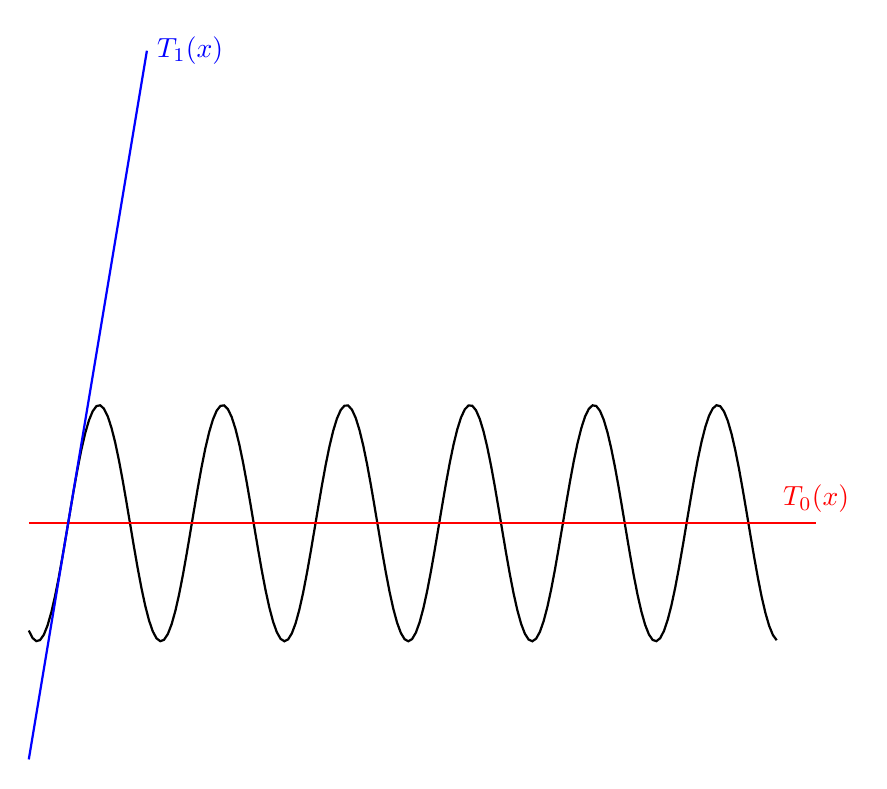
\begin{tikzpicture}
\YEaaxis{1}{10}{2}{6}
\draw[thick] plot[domain=-.5:9, samples=200](\x,{1.5*sin(4*\x r) });
\draw[thick, red] (-0.5,0)--(9.5,0) node[above]{$T_0(x)$};
\draw[thick, blue] plot[domain=-0.5:1](\x,{6*\x}) node[right]{$T_1(x)$};
\end{tikzpicture}\end{center}
\end{solution}


%%%%%%%%%%%%%%%%%%
\subsection*{\Procedural}
%%%%%%%%%%%%%%%%%%

\begin{Mquestion}
Suppose a function $f(x)$ has sixth derivative \[f^{(6)}(x)=\dfrac{6!(2x-5)}{x+3}.\] Let $T_5(x)$ be the 5th-degree Taylor polynomial for $f(x)$ about $x=11$.

Give a bound for the error
$|f(11.5)-T_5(11.5)|$.
\end{Mquestion}
\begin{hint}
In this case, Equation~\ref*{eq:taylorErrorN} tells us that
\[\left|f(11.5)-T_5(11.5)\right| = \left|\dfrac{f^{(6)}(c)}{6!}(11.5-11)^{6}\right|\] for some $c$ strictly between 11 and 11.5.
\end{hint}
\begin{answer}
$|f(11.5)-T_5(11.5)|<\dfrac{9}{7\cdot 2^6}<0.02$
\end{answer}
\begin{solution}
Equation~\ref*{eq:taylorErrorN} tells us that, when $T_n(x)$ is the $n$th degree Taylor polynomial for a function $f(x)$ about $x=a$, then
\begin{align*}
|f(x)-T_n(x)| &= \left|\frac{f^{(n+1)}(c)}{(n+1)!}(x-a)^{n+1}\right|
\intertext{for some $c$ strictly between $x$ and $a$. In our case, $n=5$, $a=11$, $x=11.5$, and $f^{(6)}(c)=\dfrac{6!(2c-5)}{c+3}$. }
\left|f(11.5)-T_5(11.5)\right|& = \left|\dfrac{1}{6!}\left(\dfrac{6!(2c-5)}{c+3}\right)(11.5-11)^{6}\right|\\
& = \left|\dfrac{2c-5}{c+3}\right|\cdot\frac{1}{2^6}
\end{align*}
for some $c$ in $(11,11.5)$. We don't know exactly which $c$ this is true for, but since we know that $c$ lies in $(11,11.5)$, we can provide bounds.
\begin{itemize}
\item $2c-5 < 2(11.5)-5=18$
\item $c+3 > 11+3=14$
\item Therefore, $\left|\dfrac{2c-5}{c+3}\right|=\dfrac{2c-5}{c+3}<\dfrac{18}{14}=\dfrac{9}{7}$ when $c \in (11,11.5)$.
\end{itemize}
With this bound, we see
\begin{align*}
|f(11.5)-T_5(11.5)| &= \left|\dfrac{2c-5}{c+3}\right|\cdot\frac{1}{2^6}\\
&<\left(\frac{9}{7}\right)\left(\frac{1}{ 2^6}\right)\approx 0.0201
\end{align*}
Our error is less than 0.02.
\end{solution}


\begin{question}
Let $f(x)= \tan x$, and let $T_2(x)$ be the second-degree Taylor polynomial for $f(x)$ about $x=0$. Give a reasonable bound on the error $|f(0.1)-T(0.1)|$ using Equation~\ref*{eq:taylorErrorN}.
\end{question}
\begin{hint}
In this case, Equation~\ref*{eq:taylorErrorN} tells us that
$\left|f(0.1)-T_2(0.1)\right| = \left|\dfrac{f^{(3)}(c)}{3!}(0.1-0)^{3}\right|$ for some $c$ strictly between 0 and 0.1.
\end{hint}
\begin{answer}
$\left|f(0.1)-T_2(0.1)\right| < \dfrac{1}{1125}$
\end{answer}
\begin{solution}
Equation~\ref*{eq:taylorErrorN} tells us that, when $T_n(x)$ is the $n$th degree Taylor polynomial for a function $f(x)$ about $x=a$, then
\begin{align*}
|f(x)-T_n(x)| &= \left|\frac{f^{(n+1)}(c)}{(n+1)!}(x-a)^{n+1}\right|
\intertext{for some $c$ strictly between $x$ and $a$. In our case, $n=2$, $a=0$, and $x=0.1$,  so }
\left|f(0.1)-T_2(0.1)\right| &= \left|\frac{f^{(3)}(c)}{3!}(0.1-0)^{3}\right|\\
&=\frac{\left|f'''(c)\right|}{6000}
\end{align*}
for some $c$ in $(0,0.1)$.

\textcolor{red}{We will find $f'''(x)$, and use it to give an upper bound for
\[\left|f(0.1)-T_2(0.1)\right|=\dfrac{\left|f'''(c)\right|}{6000}\] when  $c$ is in $(0,0.1)$.}
\begin{align*}
f(x)&=\tan x\\
f'(x)&=\sec^2 x\\
f''(x)&=2\sec x \cdot \sec x \tan x\\
&=2\sec^2 x \tan x\\
f'''(x)&=\left(2\sec^2x\right)\sec^2 x+ \left(4\sec x \cdot \sec x \tan x\right)\tan x\\
&=2\sec^4 x + 4 \sec^2 x \tan ^2 x
\end{align*}
When $0 < c < \dfrac{1}{10}$, also $0 < c < \dfrac{\pi}{6}$, so:
\begin{itemize}
\item $ \tan c < \tan\left(\dfrac{\pi}{6}\right)=\dfrac{1}{\sqrt{3}}$
\item $\cos c >\cos\left(\dfrac{\pi}{6}\right)=\dfrac{\sqrt{3}}{2}$
\item $ \sec c < \dfrac{2}{\sqrt{3}}$
\end{itemize}
With these bounds in mind for secant and tangent, we return to the expression we found for our error.
\begin{align*}
\left|f(0.1)-T_2(0.1)\right|
&=\frac{\left|f'''(c)\right|}{6000}=
\frac{\left|2\sec^4 x + 4 \sec^2 x \tan ^2 x\right|}{6000}\\
&< \frac{2\left(\frac{2}{\sqrt{3}}\right)^4+4\left(\frac{2}{\sqrt{3}}\right)^2\left(\frac{1}{\sqrt{3}}\right)^2}{6000}\\
&=\frac{1}{1125}
\end{align*}
The error is less than $\dfrac{1}{1125}$.
\end{solution}

\begin{Mquestion}
Let $f(x)=\log (1-x)$, and let $T_5(x)$ be the fifth-degree Maclaurin polynomial for $f(x)$. Use Equation~\ref*{eq:taylorErrorN} to give a bound on the error $|f\left(-\frac{1}{4}\right)-T_5\left(-\frac{1}{4}\right)|$.

(Remember $\log x=\log_ex$, the natural logarithm of $x$.)
\end{Mquestion}
\begin{hint}
In our case, Equation~\ref*{eq:taylorErrorN} tells us
\[\left|f\left(-\dfrac{1}{4}\right)-T_5\left(-\dfrac{1}{4}\right)\right| = \left|\dfrac{f^{(6)}(c)}{6!}\left(-\dfrac{1}{4}-0\right)^6\right|\]
for some $c$ between $-\dfrac{1}{4}$ and 0.
\end{hint}
\begin{answer}
$\left|f\left(-\dfrac{1}{4}\right)-T_5\left(-\dfrac{1}{4}\right)\right| < \dfrac{1}{6\cdot 4^6}<0.00004$
\end{answer}
\begin{solution}
Equation~\ref*{eq:taylorErrorN} tells us that, when $T_n(x)$ is the $n$th degree Taylor polynomial for a function $f(x)$ about $x=a$, then
\begin{align*}
|f(x)-T_n(x)| &= \left|\frac{f^{(n+1)}(c)}{(n+1)!}(x-a)^{n+1}\right|
\intertext{for some $c$ strictly between $x$ and $a$. In our case, $n=5$, $a=0$, and $x=-\dfrac{1}{4}$,  so }
\left|f\left(-\frac{1}{4}\right)-T_5\left(-\frac{1}{4}\right)\right| &= \left|\frac{f^{(6)}(c)}{6!}\left(-\frac{1}{4}-0\right)^6\right|\\
&= \frac{\left|f^{(6)}(c)\right|}{6!\cdot 4^6}
\intertext{for some $c$ in $\left(-\frac{1}{4},0\right)$. We'll need to know the sixth derivative of $f(x)$.}
f(x)&=\log (1-x)\\
f'(x)&=-(1-x)^{-1}\\
f''(x)&=-(1-x)^{-2}\\
f'''(x)&=-2(1-x)^{-3}\\
f^{(4)}(x)&=-3!(1-x)^{-4}\\
f^{(5)}(x)&=-4!(1-x)^{-5}\\
f^{(6)}(x)&=-5!(1-x)^{-6}
\intertext{Plugging in $\left|f^{(6)}(c)\right|=\dfrac{5!}{(1-c)^{6}}$:}
\left|f\left(-\frac{1}{4}\right)-T_5\left(-\frac{1}{4}\right)\right| &=
\frac{5!}{6!\cdot 4^6\cdot(1-c)^6}=\frac{1}{6\cdot 4^6 \cdot (1-c)^6}
\end{align*}
for some $c$ in $\left(-\frac{1}{4},0\right)$.

We're interested in an upper bound for the error: we want to know the worst case scenario, so we can say that the error is \emph{no worse} than that.
 We need to know what the biggest possible value of
$\dfrac{1}{6\cdot 4^6 \cdot (1-c)^6}$ is, given $-\dfrac{1}{4}<c<0$.
That means we want to know the biggest possible value of $\dfrac{1}{(1-c)^6}$. This corresponds to the smallest possible value of $(1-c)^6$, which in turn corresponds to the smallest absolute value of $1-c$.
\begin{itemize}
\item Since $-\dfrac{1}{4}\leq c \leq 0$, the smallest absolute value of $1-c$ occurs when $c=0$. In other words, $|1-c| \leq 1$.
\item  That means the smallest possible value of $(1-c)^6$ is $1^6=1$.
\item Then the largest possible value of $\dfrac{1}{(1-c)^6}$ is 1.
\item Then the largest possible value of $\dfrac{1}{6\cdot 4^6}\cdot\dfrac{1}{(1-c)^6}$ is
$\dfrac{1}{6\cdot 4^6}\approx 0.0000407$.
\end{itemize}
Finally, we conclude
\[\left|f\left(-\frac{1}{4}\right)-T_5\left(-\frac{1}{4}\right)\right| =\frac{1}{6\cdot 4^6 \cdot (1-c)^6}< \dfrac{1}{6\cdot 4^6}<0.00004\]
\end{solution}


\begin{question}
Let $f(x)=\sqrt[5]{x}$, and let $T_3(x)$ be the third-degree Taylor polynomial for $f(x)$ about $x=32$. Give a bound on the error $|f(30)-T_3(30)|$.
\end{question}
\begin{hint}
In this case, Equation~\ref*{eq:taylorErrorN} tells us that
$\left|f(30)-T_3(30)\right| = \left|\dfrac{f^{(4)}(c)}{4!}(30-32)^{4}\right|$ for some $c$ strictly between 30 and 32.

\end{hint}
\begin{answer}
Your answer may vary. One reasonable answer is\\
$\left|f(30)-T_3(30)\right|<\dfrac{14}{5^7\cdot9\cdot15}<0.000002$. Another reasonable answer is\\
$\left|f(30)-T_3(30)\right|<\dfrac{14}{5^7\cdot9}<0.00002$.
\end{answer}
\begin{solution}
Equation~\ref*{eq:taylorErrorN} tells us that, when $T_n(x)$ is the $n$th degree Taylor polynomial for a function $f(x)$ about $x=a$, then
\begin{align*}
|f(x)-T_n(x)| &= \left|\frac{f^{(n+1)}(c)}{(n+1)!}(x-a)^{n+1}\right|
\intertext{for some $c$ strictly between $x$ and $a$. In our case, $n=3$, $a=30$, and $x=32$,  so }
|f(30)-T_3(30)| &= \left|\frac{f^{(4)}(c)}{4!}(30-32)^{4}\right|\\
&=\frac{2}{3}\left|f^{(4)}(c)\right|
\end{align*}
for some $c$ in $(30,32)$.

\textcolor{red}{We will now find $f^{(4)}(x)$. Then we can give an upper bound on
$|f(30)-T_3(30)| =\dfrac{2}{3}\left|f^{(4)}(c)\right|$ when $c \in (30,32)$.}
\begin{align*}
f(x)&=x^{\tfrac{1}{5}}\\
f'(x)&=\frac{1}{5}x^{-\tfrac{4}{5}}\\
f''(x)&=-\frac{4}{5^2}x^{-\tfrac{9}{5}}\\
f'''(x)&=\frac{4\cdot 9}{5^3}x^{-\tfrac{14}{5}}\\
f^{(4)}(x)&=-\frac{4\cdot 9\cdot 14}{5^4}x^{-\tfrac{19}{5}}
\end{align*}
Using this,
\begin{align*}
|f(30)-T_3(30)|
&=\frac{2}{3}\left|f^{(4)}(c)\right|\\
&=\frac{2}{3}\left| -\frac{4\cdot 9\cdot 14}{5^4}c^{-\tfrac{19}{5}}\right|\\
&=\frac{336}{5^4\cdot c^{\tfrac{19}{5}}}
\intertext{Since $30 < c< 32$,}
&< \frac{336}{5^4\cdot 30^{\tfrac{19}{5}}}
=\frac{336}{5^4\cdot 30^3 \cdot 30^{\tfrac{4}{5}}}\\
&=\frac{14}{5^7\cdot 9 \cdot 30^{\tfrac{4}{5}}}
\intertext{This isn't a number we know. We're trying to find the error in our estimation of $\sqrt[5]{30}$, but $\sqrt[5]{30}$ shows up in our error. From here, we have to be a little creative to get a bound that actually makes sense to us. There are different ways to go about it.
You could simply use $30^{\tfrac{4}{5}}>1$. We will be a little more careful, and
use the following estimation:}
\frac{14}{5^7 \cdot 9 \cdot \textcolor{red}{30^{\tfrac{4}{5}}}}&=
\frac{14\cdot \textcolor{red}{30^{\tfrac{1}{5}}}}{5^7 \cdot 9 \cdot \textcolor{red}{30}}\\
&<\frac{14\cdot \textcolor{red}{32^{\tfrac{1}{5}}}}{5^7 \cdot 9 \cdot \textcolor{red}{30}}\\
&<\frac{14\cdot \textcolor{red}{2}}{5^7 \cdot 9 \cdot \textcolor{red}{30}}\\
&<\frac{14}{5^7\cdot 9 \cdot \textcolor{red}{15}}\\
&< 0.000002
\end{align*}
We conclude $\left|f(30)-T_3(30)\right|<0.000002$.
\end{solution}




\begin{question}
Let \[f(x)= \sin\left(\dfrac{1}{x}\right),\] and let $T_1(x)$ be the first-degree Taylor polynomial for $f(x)$ about $x=\dfrac{1}{\pi}$. Give a bound on the error $|f(0.01)-T_1(0.01)|$, using Equation~\ref*{eq:taylorErrorN}. You may leave your answer in terms of $\pi$.

Then, give a \emph{reasonable} bound on the error $|f(0.01)-T_1(0.01)|$.
\end{question}
\begin{hint}
In our case, Equation~\ref*{eq:taylorErrorN} tells us\\
$\left|f\left(0.01\right)-T_1\left(0.01\right)\right| = \left|\dfrac{f^{(2)}(c)}{2!}\left(0.01-\frac{1}{\pi}\right)^2\right|$ for some $c$ between 0.01 and $\dfrac{1}{\pi}$.
\end{hint}
\begin{answer}
Equation~\ref*{eq:taylorErrorN}  gives the bound
$|f(0.01)-T_n(0.01)| \leq 100^2\left(\frac{100}{\pi}-1\right)^2$.

A more reasonable bound on the error is that it is less than 5.
\end{answer}
\begin{solution}
Equation~\ref*{eq:taylorErrorN} tells us that, when $T_n(x)$ is the $n$th degree Taylor polynomial for a function $f(x)$ about $x=a$, then
\begin{align*}
|f(x)-T_n(x)| &= \left|\frac{f^{(n+1)}(c)}{(n+1)!}(x-a)^{n+1}\right|
\intertext{for some $c$ strictly between $x$ and $a$. In our case, $n=1$, $a=\dfrac{1}{\pi}$, and $x=0.01$,  so }
|f(0.01)-T_1(0.01)| &= \left|\frac{f''(c)}{2}\left(0.01-\frac{1}{\pi}\right)^{2}\right|\\
&=\frac{1}{2}\left(\frac{100-\pi}{100\pi}\right)^2\cdot\left|f''(c)\right|
\end{align*}
for some $c$ in $\left(\frac{1}{100},\frac{1}{\pi}\right)$.

Let's find $f''(x)$.
\begin{align*}
f(x)&=\sin\left(\frac{1}{x}\right)\\
f'(x)&=\cos\left(\frac{1}{x}\right)\cdot\frac{-1}{x^2}=\frac{-\cos\left(\frac{1}{x}\right)}{x^2}\\
f''(x)&=\frac{x^2\sin\left(\frac{1}{x}\right)(-x^{-2})+\cos\left(\frac{1}{x}\right)(2x)}{x^4}\\
&=\frac{2x\cos\left(\frac{1}{x}\right)-\sin\left(\frac{1}{x}\right)}{x^4}
\end{align*}

Now we can plug in a better expression for $f''(c)$:
\begin{align*}
|f(0.01)-T_1(0.01)| &=\frac{1}{2}\left(\frac{100-\pi}{200\pi}\right)^2\cdot\left|f''(c)\right|\\
&=\frac{1}{2}\left(\frac{100-\pi}{100\pi}\right)^2\cdot
\frac{\left|2c\cos\left(\frac{1}{c}\right)-\sin\left(\frac{1}{c}\right)\right|}{c^4}
\intertext{for some $c$ in $\left(\frac{1}{100},\frac{1}{\pi}\right)$.}
\end{align*}
\textcolor{red}{What we want to do now is find an upper bound on this expression containing $c$,\\
$\dfrac{1}{2}\left(\dfrac{100-\pi}{100\pi}\right)^2\cdot
\dfrac{\left|2c\cos\left(\frac{1}{c}\right)-\sin\left(\frac{1}{c}\right)\right|}{c^4}$
.}
\begin{itemize}
\item Since $c \geq \dfrac{1}{100}$, it follows that $c^4 \geq \dfrac{1}{100^4}$, so
$\dfrac{1}{c^4}\leq 100^4$.
\item For any value of $x$, $|\cos x|$ and $|\sin x|$ are at most 1.
Since $|c|<1$, also $|c\cos\left(\frac{1}{c}\right)| <|\cos\left(\frac{1}{c}\right)|  \leq 1$.
 So,
$\left|2c\cos\left(\frac{1}{c}\right)-\sin\left(\frac{1}{c}\right)\right| < 3$
\item Therefore,
\begin{align*}
|f(0.01)-T_n(0.01)|=&\,\dfrac{1}{2}\left(\dfrac{100-\pi}{100\pi}\right)^2\cdot\frac{1}{c^4}\cdot
\left|2c\cos\left(\frac{1}{c}\right)-\sin\left(\frac{1}{c}\right)\right|\\
<
&\,\dfrac{1}{2}\left(\dfrac{100-\pi}{100\pi}\right)^2\cdot100^4\cdot3\\
=&\,\frac{3\cdot 100^2}{2}\left(\frac{100}{\pi}-1\right)^2\\
\end{align*}
\end{itemize}
Equation~\ref*{eq:taylorErrorN}  gives the bound
$|f(0.01)-T_1(0.01)| \leq \frac{3\cdot 100^2}{2}\left(\frac{100}{\pi}-1\right)^2$.


The bound above works out to approximately fourteen million. One way to understand why the bound is so high is that $\sin\left(\frac{1}{x}\right)$ moves about crazily when $x$ is near zero--it moves up and down incredibly fast, so a straight line isn't going to approximate it very well at all.

That being said, because $\sin\left(\frac{1}{x}\right)$ is still ``sine of something," we know $-1 \leq f\left(0.01\right) \leq 1$. To get a better bound on the error, let's find $T_1(x)$.
\begin{align*}
f(x)&=\sin\left(\frac{1}{x}\right)
&
f\left(\frac{1}{\pi}\right)&=\sin(\pi)=0\\
f'(x)&=\frac{-\cos\left(\frac{1}{x}\right)}{x^2} &
f'\left(\frac{1}{\pi}\right)&=-\pi^2\cos(\pi)=\pi^2\end{align*}
\begin{align*}
T_1(x)&=f\left(\frac{1}{\pi}\right)+f'\left(\frac{1}{\pi}\right)\left(x-\frac{1}{\pi}\right)\\
&=0+\pi^2\left(x-\frac{1}{\pi}\right)\\&=\pi^2x-\pi\\
T_1\left(0.01\right)& = \frac{\pi^2}{100}-\pi
\end{align*}
Now that we know $T_1(0.01)$, and we know $-1 \leq f(0.01) \leq 1$, we can give the bound
\begin{align*}
\left|f(0.01)-T_1(0.01)\right|&\leq
\left|f(0.01)\right|+\left|T_1(0.01)\right|\\
&\leq 1 +\left| \frac{\pi^2}{100}-\pi\right|\\
&=1+\pi\left|1-\frac{\pi}{100}\right|\\
&<1+\pi\\
&<1+4=5
\end{align*}
A more reasonable bound on the error is that it is less than 5.

Still more reasonably, we would not use $T_1(x)$ to
           evaluate $\sin(100)$ approximately.  We would write
           $\sin(100) = \sin(100-32\pi)$ and approximate the right
           hand side, which is roughly $\sin(-\pi/6)$.
\end{solution}










\begin{Mquestion}
Let $f(x)=\arcsin x$, and let $T_2(x)$ be the second-degree Maclaurin polynomial for $f(x)$. Give a reasonable bound on the error $\left|f\left(\frac{1}{2}\right)-T_2\left(\frac{1}{2}\right)\right|$
using Equation~\ref*{eq:taylorErrorN}. What is the exact value of the error $\left|f\left(\frac{1}{2}\right)-T_2\left(\frac{1}{2}\right)\right|$?
\end{Mquestion}
\begin{hint}
Using Equation~\ref*{eq:taylorErrorN},
$\left|f\left(\dfrac{1}{2}\right)-T_2\left(\dfrac{1}{2}\right)\right| = \left|\dfrac{f^{(3)}(c)}{3!}\left(\dfrac{1}{2}-0\right)^{3}\right|$ for some $c$ in $\left(0,\dfrac{1}{2}\right)$.
\end{hint}
\begin{answer}
Using Equation~\ref*{eq:taylorErrorN},
\begin{align*}
\left|f\left(\frac{1}{2}\right)-T_2\left(\frac{1}{2}\right)\right|&<\frac{1}{10}.
\intertext{The actual error is}
\left|f\left(\frac{1}{2}\right)-T_2\left(\frac{1}{2}\right)\right|&= \frac{\pi}{6}-\frac{1}{2}\end{align*}
which is about 0.02.
\end{answer}
\begin{solution}
Equation~\ref*{eq:taylorErrorN} tells us that, when $T_n(x)$ is the $n$th degree Taylor polynomial for a function $f(x)$ about $x=a$, then
\begin{align*}
|f(x)-T_n(x)| &= \left|\frac{f^{(n+1)}(c)}{(n+1)!}(x-a)^{n+1}\right|
\intertext{for some $c$ strictly between $x$ and $a$. In our case, $n=2$, $a=0$, and $x=\dfrac{1}{2}$,  so }
\left|f\left(\frac{1}{2}\right)-T_2\left(\frac{1}{2}\right)\right| &= \left|\frac{f^{(3)}(c)}{3!}\left(\frac{1}{2}-0\right)^{3}\right|\\
&= \frac{\left|f^{(3)}(c)\right|}{3!\cdot2^3}
\end{align*}
for some $c$ in $\left(0,\frac{1}{2}\right)$.\\
\textcolor{red}{ The next task that suggests itself is finding $f^{(3)}(x)$.}
\begin{align*}
f(x)&=\arcsin x\\
f'(x)&=\frac{1}{\sqrt{1-x^2}}=(1-x^2)^{-\tfrac{1}{2}}\\
f''(x)&=-\frac{1}{2}(1-x^2)^{-\tfrac{3}{2}}(-2x)\\
&=x(1-x^2)^{-\tfrac{3}{2}}\\
f'''(x)&=x\left(-\frac{3}{2}\right)(1-x^2)^{-\tfrac{5}{2}}(-2x)+(1-x^2)^{-\tfrac{3}{2}}\\
&=3x^2(1-x^2)^{-\tfrac{5}{2}}+(1-x^2)^{-\tfrac{5}{2}+1}\\
&=(1-x^2)^{-\tfrac{5}{2}}\left(3x^2+(1-x^2)\right)\\
&=(1-x^2)^{-\tfrac{5}{2}}\left(2x^2+1\right)
\intertext{Since  $\left|f\left(\frac{1}{2}\right)-T_2\left(\frac{1}{2}\right)\right| =\dfrac{\left|f^{(3)}(c)\right|}{3!\cdot2^3}$ for some $c$ in $\left(0,\frac{1}{2}\right)$,}
\left|f\left(\frac{1}{2}\right)-T_2\left(\frac{1}{2}\right)\right| &=\dfrac{\left|\dfrac{1+2c^2}
{\left(\sqrt{1-c^2}\right)^5}
\right|}{3!\cdot2^3}=
\frac{1+2c^2}{48\left(\sqrt{1-c^2}\right)^5}
\intertext{for some $c$ in $\left(0,\frac{1}{2}\right)$.}
\end{align*}
 We want to know what is the worst case scenario-what's the biggest this expression can be.
 \textcolor{red}{So, now we find an upper bound on $\dfrac{1+2c^2}{48\left(\sqrt{1-c^2}\right)^5}$ when $0 \leq c \leq \dfrac{1}{2}$.}
  Remember that our bound doesn't have to be exact, but it should be relatively easy to calculate.
\begin{itemize}
\item When $0 \leq c \leq\dfrac{1}{2}$, the biggest $1+2c^2$ can be is $1+2\left(\dfrac{1}{2}\right)^2=\dfrac{3}{2}$.\\ So, the \textcolor{red}{numerator} of $\dfrac{1+2c^2}{48\left(\sqrt{1-c^2}\right)^5}$ is at most $\dfrac{3}{2}$.
\item The smallest $1-c^2$ can be is $1-\left(\dfrac{1}{2}\right)^2=\dfrac{3}{4}$.
\item So, the smallest $\left(\sqrt{1-c^2}\right)^5$ can be is
$\left(\sqrt{\dfrac{3}{4}}\right)^5=\left(\dfrac{\sqrt{3}}{2}\right)^5$.
\item Then smallest possible value for the \textcolor{red}{denominator} of $\dfrac{1+2c^2}{48\left(\sqrt{1-c^2}\right)^5}$ is $48\left(\dfrac{\sqrt{3}}{2}\right)^5$
\item Then
\begin{align*}
\dfrac{1+2c^2}{48\left(\sqrt{1-c^2}\right)^5}
& \leq \frac{\dfrac{3}{2}}{48\left(\dfrac{\sqrt{3}}{2}\right)^5}\\
&=\frac{1}{\sqrt{3}^5}=\frac{1}{9\sqrt{3}}\\
&<\frac{1}{10}
\end{align*}
\end{itemize}
Let's put together these pieces. We found that
\[\left|f\left(\frac{1}{2}\right)-T_2\left(\frac{1}{2}\right)\right| =\frac{1+2c^2}{48\left(\sqrt{1-c^2}\right)^5}\]
for some $c$ in $\left(0,\frac{1}{2}\right)$. We also found that
\[\frac{1+2c^2}{48\left(\sqrt{1-c^2}\right)^5}<\frac{1}{10}\]
when $c$ is in $\left(0,\frac{1}{2}\right)$.
We conclude
\[\left|f\left(\frac{1}{2}\right)-T_2\left(\frac{1}{2}\right)\right|<\frac{1}{10}.\]

\textcolor{blue}{For the second part of the question, we need to find $f\left(\frac{1}{2}\right)$ and $T_2\left(\frac{1}{2}\right)$.}\\
 Finding $f\left(\frac{1}{2}\right)$ is not difficult.
\begin{align*}
f(x)&=\arcsin x\\
f\left(\frac{1}{2}\right)&=\arcsin\left(\frac{1}{2}\right)=\frac{\pi}{6}
\end{align*}
\textcolor{blue}{In order to find $T_2\left(\frac{1}{2}\right)$, we need to find $T_2(x)$.}
\begin{align*}
T_2(x)&=f(0)+f'(0)x+\frac{1}{2}f''(0)x^2
\intertext{Conveniently, we've already found the first few derivatives of $f(x)$.}
T_2(x)&=\arcsin(0)+\left(\frac{1}{\sqrt{1-0^2}}\right)x+\frac{1}{2}\left(\frac{0}{\left(\sqrt{1-0^2}\right)^3}\right)x^2\\
&=0+x+0\\
&=x\\
T_2\left(\frac{1}{2}\right)&=\frac{1}{2}
\intertext{So, the actual error is}
\left|f\left(\frac{1}{2}\right)-T_2\left(\frac{1}{2}\right)\right|&=\left| \frac{\pi}{6}-\frac{1}{2}\right|= \frac{\pi}{6}-\frac{1}{2}
\end{align*}
A calculator tells us that this is about 0.02.
\end{solution}





%%%%%%%%%%%%%%%%%%
\subsection*{\Application}
%%%%%%%%%%%%%%%%%%


\begin{question}
Let $f(x)=\log(x)$, and let $T_n(x)$ be the $n$th-degree Taylor polynomial for $f(x)$ about
$x=1$. You use $T_n(1.1)$ to estimate $\log (1.1)$.
If your estimation needs to have an error of no more than $10^{-4}$, what is an acceptable value of $n$ to use?
\end{question}
\begin{hint}
It helps to have a formula for $f^{(n)}(x)$. You can figure it out by taking several derivatives and noticing the pattern, but also this has been given previously in the text.
\end{hint}
\begin{answer}
Any $n$ greater than or equal to 3.
\end{answer}
\begin{solution}
Our error will have the form $\dfrac{f^{(n+1)}(c)}{(n+1)!}(x-1)^{n+1}$ for some constant $c$, so let's find an equation for $f^{(n)}(x)$. This has been done before in the text, but we'll do it again here: we'll take several derivatives, then notice the pattern.
\begin{align*}
f(x)&=\log x\\
f'(x)&=x^{-1}\\
f''(x)&=-x^{-2}\\
f'''(x)&=2!\,x^{-3}\\
f^{(4)}(x)&=-3!\,x^{-4}\\
f^{(5)}(x)&=4!\,x^{-5}
\intertext{So, when $n \geq 1$,}
f^{(n)}(x)&=(-1)^{n-1}(n-1)!\cdot x^{-n}
\end{align*}
Now that we know the derivative of $f(x)$, we have a better idea what the error in our approximation looks like.
\begin{align*}
\left|f(1.1)-T_n(1.1)\right|&=\left|\dfrac{f^{(n+1)}(c)}{(n+1)!}(1.1-1)^{n+1}\right|\\
&=\left|f^{(n+1)}(c)\right|\frac{0.1^{n+1}}{(n+1)!}\\
&=\left|\frac{n!}{c^{n+1}}
\right|\frac{1}{10^{n+1}(n+1)!}\\
&=\frac{1}{ |c|^{n+1}\cdot10^{n+1}\cdot(n+1)}
\intertext{for some $c$ in $(1,1.1)$}
&<\frac{1}{(n+1)10^{n+1}\cdot 1^{n+1}}\\
&=\frac{1}{(n+1)10^{n+1}}
\intertext{What we've shown so far is }
|f(1.1)-T_n(1.1)|&<\dfrac{1}{(n+1)10^{n+1}}
\intertext{If we can show that $\dfrac{1}{(n+1)10^{n+1}}\le10^{-4}$, then we'll be able to conclude}
|f(1.1)-T_n(1.1)|&<\dfrac{1}{(n+1)10^{n+1}}\le10^{-4}
\end{align*}
That is, our error is less than $10^{-4}$.

So, our goal for the problem is to find a value of $n$ that makes $\dfrac{1}{(n+1)10^{n+1}}\le10^{-4}$. Certainly, $n=3$ is such a number. Therefore,  any $n$ greater than or equal to 3 is an acceptable value.
\end{solution}


\begin{Mquestion}
Give an estimation of $\sqrt[7]{2200}$ using a Taylor polynomial. Your estimation should have an error of less than 0.001.
\end{Mquestion}
\begin{hint}
You can approximate the function $f(x)=x^{\tfrac{1}{7}}$.\\ It's a good bit of trivia to know $3^7=2187$.\\
A low-degree Taylor approximation will give you a good enough estimation.
If you guess a degree, and take that Taylor polynomial, the error will \emph{probably} be less than 0.001 (but you still need to check).
\end{hint}
\begin{answer}
$\sqrt[7]{2200}\approx3+\dfrac{13}{7\cdot 3^6}
\approx 3.00255$
\end{answer}
\begin{solution}
We will approximate $f(x)=x^{\tfrac{1}{7}}$ using a Taylor polynomial. Since $3^7=2187$, we will use $x=2187$ as our centre.

 \textcolor{red}{We need to figure out which degree Taylor polynomial will result in a  small-enough error. }

If we use the $n$th Taylor polynomial, our error will be
\begin{align*}
\left|f(2200)-T_n(2200)\right|&=\left|\frac{f^{(n+1)}(c)}{(n+1)!}(2200-2187)^{n+1}\right|\\
&=\left|f^{(n+1)}(c)\right|\cdot\frac{13^{n+1}}{(n+1)!}
\intertext{for some $c$ in $(2187,2200)$. In order for this to be less than 0.001, we need}
\left|f^{(n+1)}(c)\right|\cdot\frac{13^{n+1}}{(n+1)!}&<0.001\\
\left|f^{(n+1)}(c)\right|&<\frac{ (n+1)!}{1000\cdot13^{n+1}}
\end{align*}
It's a tricky thing to figure out which $n$ makes this true. Let's make a table. We won't show all the work of filling it in, but the work is standard.

\begin{displaymath}
\begin{array}{c|c|c|c}
n & \dfrac{(n+1)!}{1000\cdot 13^{n+1}}
&
\left|f^{(n+1)}(c)\right|
&
\textup{Is }\left|f^{(n+1)}(c)\right|<\dfrac{ (n+1)!}{1000\cdot13^{n+1}}\textup{?}
\\~&~&~\\
\hline
~&~&~\\
0&\dfrac{1}{1000\cdot 13}&|f'(c)|=\dfrac{1}{7c^{6/7}}<\dfrac{1}{7\cdot 3^6}&
\\~&~&~\\
\hline
~&~&~\\
1&\dfrac{2}{1000\cdot 13^2}&|f''(c)|=\dfrac{6}{7^2\cdot c^{\tfrac{13}{7}}}<\dfrac{6}{7^2\cdot 3^{13}}&\textup{Yes!}
\end{array}\end{displaymath}

That is: if we use the first-degree Taylor polynomial, then for some $c$ between $2187$ and $2200$,
\begin{align*}
|f(2200)-T_1(2200)|&=\left|f''(c)\right|\cdot\frac{13^2}{2!}\\
&=\frac{6}{7^2\cdot c^{\tfrac{13}{7}}}\cdot\frac{13^2}{2}\\
&<\dfrac{6}{7^2\cdot 3^{13}}\cdot\dfrac{13^2}{2}\\
&=\dfrac{3\cdot 13^2}{7^2 \cdot 3^{13}}\approx 0.0000065
\end{align*}

So, actually, the linear Taylor polynomial (or any higher-degree Taylor polynomial) will result in an approximation that is much more accurate than required. (We don't know, however, that the constant approximation will be accurate enough--so we'd better stick with $n \geq 1$.)

\textcolor{red}{Now that we know we can take the first-degree Taylor polynomial, let's compute $T_1(x)$.} Recall we are taking the Taylor polynomial for $f(x)=x^{\tfrac{1}{7}}$ about $x=2187$.
\begin{align*}
f(2187)&=2187^{\tfrac{1}{7}}=3\\
f'(x)&=\frac{1}{7}x^{-\tfrac{6}{7}}\\
f'(2187)&=\frac{1}{7\sqrt[7]{2187}^6}=\frac{1}{7\cdot3^6}\\
T_1(x)&=f(2187)+f'(2187)(x-2187)\\
&=3+\frac{x-2187}{7\cdot3^6}\\
T_1(2200)&=3+\frac{2200-2187}{7\cdot3^6}\\
&=3+\frac{13}{7\cdot 3^6}\\
&\approx 3.00255
\end{align*}
We conclude $\sqrt[7]{2200}\approx 3.00255$.
\end{solution}


\begin{question}
Use Equation~\ref*{eq:taylorErrorN} to show that
\[\frac{4241}{5040}\leq\sin(1) \leq\frac{4243}{5040}\]
\end{question}
\begin{hint}
Use the 6th-degree Maclaurin approximation for $f(x)=\sin x$.
\end{hint}
\begin{answer}
If we're going to use  Equation~\ref*{eq:taylorErrorN}, then we'll probably be taking a Taylor polynomial. Using Example~\ref*{eg expand sinx}, %3.4.16
the 6th-degree Maclaurin polynomial for $\sin x$ is
\[T_6(x)=T_5(x)=x-\frac{x^3}{3!}+\frac{x^5}{5!}\]
so let's play with this a bit. Equation~\ref*{eq:taylorErrorN} tells us that the error will depend on the seventh derivative of $f(x)$, which is $-\cos x$:
\begin{align*}
f(1)-T_6(1)&=f^{(7)}(c)\frac{1^7}{7!}\\
\sin(1)-\left(1-\frac{1}{3!}+\frac{1}{5!}\right)&=\frac{-\cos c}{7!}\\
\sin(1)-\frac{101}{5!}&=\frac{-\cos c}{7!}\\
\sin(1)&=\frac{4242-\cos c}{7!}
\intertext{for some $c$ between 0 and 1. Since $-1 \leq \cos c \leq 1$,}
\frac{4242-1}{7!}\leq \sin(1)&\leq \frac{4242+1}{7!}\\
\frac{4241}{7!}\leq \sin(1)&\leq \frac{4243}{7!}\\
\frac{4241}{5040}\leq \sin(1)&\leq \frac{4243}{5040}\\
\end{align*}

Remark: there are lots of ways to play with this idea to get better estimates. One way is to take a higher-degree Maclaurin polynomial. Another is to note that, since $0<c<1<\dfrac{\pi}{3}$, then $\dfrac{1}{2}<\cos c < 1$, so
\begin{align*}
\dfrac{4242-1}{7!}<\sin(1)<\dfrac{4242-\frac{1}{2}}{7!}\\
\dfrac{4241}{5040}<\sin(1)<\dfrac{8483}{10080}<\frac{4243}{5040}
\end{align*}
If you got tighter bounds than asked for in the problem, congratulations!
\end{answer}
\begin{solution}
If we're going to use  Equation~\ref*{eq:taylorErrorN}, then we'll probably be taking a Taylor polynomial. Using Example~\ref*{eg expand sinx}, %3.4.16
the 6th-degree Maclaurin polynomial for $\sin x$ is
\[T_6(x)=T_5(x)=x-\frac{x^3}{3!}+\frac{x^5}{5!}\]
so let's play with this a bit. Equation~\ref*{eq:taylorErrorN} tells us that the error will depend on the seventh derivative of $f(x)$, which is $-\cos x$:
\begin{align*}
f(1)-T_6(1)&=f^{(7)}(c)\frac{1^7}{7!}\\
\sin(1)-\left(1-\frac{1}{3!}+\frac{1}{5!}\right)&=\frac{-\cos c}{7!}\\
\sin(1)-\frac{101}{5!}&=\frac{-\cos c}{7!}\\
\sin(1)&=\frac{4242-\cos c}{7!}
\intertext{for some $c$ between 0 and 1. Since $-1 \leq \cos c \leq 1$,}
\frac{4242-1}{7!}\leq \sin(1)&\leq \frac{4242+1}{7!}\\
\frac{4241}{7!}\leq \sin(1)&\leq \frac{4243}{7!}\\
\frac{4241}{5040}\leq \sin(1)&\leq \frac{4243}{5040}\\
\end{align*}

Remark: there are lots of ways to play with this idea to get better estimates. One way is to take a higher-degree Maclaurin polynomial. Another is to note that, since $0<c<1<\dfrac{\pi}{3}$, then $\dfrac{1}{2}<\cos c < 1$, so
\begin{align*}
\dfrac{4242-1}{7!}<\sin(1)<\dfrac{4242-\frac{1}{2}}{7!}\\
\dfrac{4241}{5040}<\sin(1)<\dfrac{8483}{10080}<\frac{4243}{5040}
\end{align*}
If you got tighter bounds than asked for in the problem, congratulations!
\end{solution}


%%%
%%% Andrew - extra problem starts here.
%%%

\begin{question}
In this question, we use the remainder of a Maclaurin polynomial to approximate $e$.
\begin{enumerate}[(a)]
\item\label{s3.4.8T(x)} Write out the 4th degree Maclaurin polynomial $T_4(x)$ of the function $e^x$.
\item\label{s3.4.8T(1)} Compute $T_4(1)$.
\item\label{s3.4.8(e)} Use your answer from \ref{s3.4.8T(1)} to conclude $\dfrac{326}{120}<e<\dfrac{325}{119}$.
\end{enumerate}
\end{question}
\begin{hint}
For part \eqref{s3.4.8(e)}, after you plug in the appropriate values to Equation~\ref*{eq:taylorErrorN}, simplify the upper and lower bounds for $e$ separately. In particular, for the upper bound, you'll have to solve for $e$.
\end{hint}
\begin{answer}
(a) $T_4(x)=\sum_{n=0}^4\frac{x^n}{n!}$\qquad
(b) $T_4(1)=\frac{65}{24}$\qquad
(c) See the solution.
\end{answer}
\begin{solution}
\eqref{s3.4.8T(x)}
For every whole number $n$, the $n$th derivative of $e^x$ is $e^x$. So:
\[
T_4(x)=\sum_{n=0}^4\frac{e^0}{n!}x^n
=\sum_{n=0}^4\frac{x^n}{n!}\]


\eqref{s3.4.8T(1)}
\begin{align*}
T_4(1)&=\sum_{n=0}^4\frac{1^n}{n!}=\sum_{n=0}^4\frac{1}{n!}\\
&=\frac{1}{0!}+\frac{1}{1!}+\frac{1}{2!}+\frac{1}{3!}+\frac{1}{4!}\\
&=\frac{1}{1}+\frac{1}{1}+\frac{1}{2}+\frac{1}{6}+\frac{1}{24}\\
&=\frac{65}{24}
\end{align*}

\eqref{s3.4.8(e)} Using Equation~\ref*{eq:taylorErrorN},
\begin{align*}
e^1-T_4(1)&=\frac{1}{5!}e^c\qquad\mbox{for some $c$ strictly between 0 and 1. So,}\\
e-\frac{65}{24}&=\frac{e^c}{120}\\
e&=\frac{65}{24}	+\frac{e^c}{120}
\intertext{Since $e^x$ is a strictly increasing function, and $0<c<1$, we conclude $e^0<e^c<e^1$:}
\frac{65}{24}	+\frac{1}{120}& <e<\frac{65}{24}	+\frac{e}{120}
\intertext{Simplifying the left inequality, we see}
\frac{326}{120}&<e
\intertext{From the right inequality, we see}
e&<\frac{65}{24}+\frac{e}{120}\\
e-\frac{e}{120}&<\frac{65}{24}\\
e\cdot \frac{119}{120}&<\frac{65}{24}\\
e&<\frac{65}{24}\cdot \frac{120}{119}=\frac{325}{119}
\intertext{So, we conclude}
\frac{326}{120}&<e<\frac{325}{119},
\end{align*}
as desired.

Remark: $\dfrac{326}{120}\approx 2.717$, and
$\dfrac{325}{119}\approx 2.731$.

\end{solution}

%%%
%%% Andrew - extra problem ends here.
%%%
